
\tikzset{
	path image1/.style={
		path picture={
			\node at (path picture bounding box.center) {
				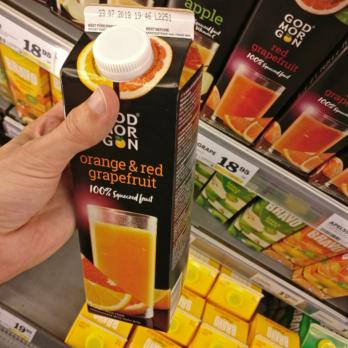
\includegraphics[height=2cm]{Chapter3/tikz/God-Morgon-Orange-Red-Grapefruit-Juice_002.jpg}};}},
	path image2/.style={
		path picture={
			\node at (path picture bounding box.center) {
				
\includegraphics[height=1.5cm]{Chapter3/tikz/God-Morgon-Orange-Red-Grapefruit-Juice_Iconic.jpg}};}},
}

\begin{tikzpicture}
    \node[font=\sffamily] at (1,2.25) {\begin{tabular}{c}Input image $\boldsymbol{I}$ \end{tabular}};
\draw[path image1,draw=black, thick] (0,0) rectangle (2,2);

\node[fill=Green!20, minimum width=0.5cm, minimum height=1.5cm, draw] (x) at (5.25cm,1) {\large $\boldsymbol x$};
\node[font=\sffamily] at (5.25cm,2.25) {\begin{tabular}{c}Feature vector $\boldsymbol{x}$ \\ of image $\boldsymbol{I}$ \end{tabular}};

\draw[fill=orange!20] ([xshift=-0.5cm]x.north west) -- ([xshift=-2.5cm,yshift=1.0cm]x.west) -- ([xshift=-2.5cm,yshift=-1.0cm]x.west) -- ([xshift=-0.5cm]x.south west) -- cycle;
\node at (3.5,1.25) {{\sf \textbf{Pretrained}}};
\node at (3.5,0.75) {{\sf \textbf{CNN} $f_{\boldsymbol{\varphi}}(\boldsymbol{I})$}};

\draw[fill=Green!20] ([xshift=0.5cm]x.north east) -- ([xshift=2.5cm,yshift=0.25cm]x.east) -- ([xshift=2.5cm,yshift=-0.25cm]x.east) -- ([xshift=0.5cm]x.south east) -- cycle; 
\node at (7.0,1.0) {\large $q_{\boldsymbol{\phi}}(\boldsymbol{z} | \boldsymbol{x})$};

\node[fill=red!20, minimum width=0.5cm, minimum height=0.75cm, draw] (z) at (8.75cm,1.0) {\large $\boldsymbol z$};
\node[font=\sffamily] at (8.5cm,1.9) {\begin{tabular}{c}Shared \\ latent $\boldsymbol{z}$ \end{tabular}};


\node[fill=blue!20, minimum width=0.5cm, minimum height=1.5cm, draw] (xhat) at (12.25cm,1) {\large $\boldsymbol{\hat{x}}$};
\node[font=\sffamily] at (14.25cm,1) {\begin{tabular}{c}Feature vector $\boldsymbol{\hat{x}} \approx \boldsymbol{x}$ \\ of image $\boldsymbol{I}$ \end{tabular}};


\draw[fill=blue!20] ([xshift=0.5cm]z.north east) -- ([xshift=-0.5cm,yshift=0.75cm]xhat.west) -- ([xshift=-0.5cm,yshift=-0.75cm]xhat.west) -- ([xshift=0.5cm]z.south east) -- cycle; 
\node at (10.5,1.0) {\large $p_{\boldsymbol{\theta_x}}(\boldsymbol{x} | \boldsymbol{z})$};

\draw[path image2,draw=black, thick] (12,2.25) rectangle (13.5,3.75);

\draw[fill=blue!20] ([xshift=0.5cm,yshift=2.cm]z.north east) -- ([xshift=2.5cm,yshift=2.75cm]z.east) -- ([xshift=2.5cm,yshift=1.25cm]z.east) -- ([xshift=0.5cm,yshift=2.cm]z.south east) -- cycle; 
\node at (10.5,3.0) {\large $p_{\boldsymbol{\theta_i}}(\boldsymbol{i} | \boldsymbol{z})$};

\node[font=\sffamily] at (14.75cm,3) {\begin{tabular}{c}Iconic image $\boldsymbol{i}$\end{tabular}};

\node[draw,text width=5.25cm,font=\sffamily\itshape] (text) at (14.75cm,-1) {\small{"God Morgon Orange/Red Grapefruit is a fresh blend of sweet orange juice and tasty fresh red grapefruit."}};
\draw[fill=blue!20] ([xshift=0.5cm,yshift=-2.cm]z.north east) -- ([xshift=2.5cm,yshift=-1.25cm]z.east) -- ([xshift=2.5cm,yshift=-2.75cm]z.east) -- ([xshift=0.5cm,yshift=-2.cm]z.south east) -- cycle; 
\node at (10.5,-1.0) {\large $p_{\boldsymbol{\theta_w}}(\boldsymbol{w} | \boldsymbol{z})$};
\node[font=\sffamily] at (14.5cm,-0.1) {\begin{tabular}{c}Text description $\boldsymbol{w}$\end{tabular}};

\node[draw,text width=3.75cm,font=\sffamily] (label) at (14.cm,-3.) {God Morgon Orange and Red Grapefruit Juice};
\draw[fill=blue!20] ([xshift=0.5cm,yshift=-4.0cm]z.north east) -- ([xshift=2.5cm,yshift=-3.25cm]z.east) -- ([xshift=2.5cm,yshift=-4.75cm]z.east) -- ([xshift=0.5cm,yshift=-4.0cm]z.south east) -- cycle; 
\node at (10.5,-3.0) {\large $p_{\boldsymbol{\theta_y}}(\boldsymbol{y} | \boldsymbol{z})$};
\node[font=\sffamily] at (14.cm,-2.3) {\begin{tabular}{c}Class label $\boldsymbol{y}$\end{tabular}};

% Softmax classifier
\node[draw,text width=3.75cm,font=\sffamily] (label1) at (5.75cm,-3.) {God Morgon Orange and Red Grapefruit Juice};
\node[fill=red!20, minimum width=0.5cm, minimum height=0.75cm, draw] (z1) at (1.0cm,-3) {\large $\boldsymbol z$};
\draw[fill=orange!20] ([xshift=0.5cm]z1.north east) -- ([xshift=2.cm,yshift=0.75cm]z1.east) -- ([xshift=2.cm,yshift=-0.75cm]z1.east) -- ([xshift=0.5cm]z1.south east) -- cycle; 
\node at (2.5,-3) {\large $f_{\boldsymbol{\lambda}}(\boldsymbol{z})$};
\node[font=\sffamily] at (5.75cm,-2.3) {\begin{tabular}{c}Class label $\boldsymbol{y}$\end{tabular}};

\draw[draw=black, thick, rounded corners, dashed] ([xshift=-0.5cm,yshift=0.75cm]z1.north west) -- ([xshift=7.5cm, yshift=0.75cm]z1.north west) -- ([xshift=7.5cm,yshift=-0.75cm]z1.south west) -- ([xshift=-0.5cm,yshift=-0.75cm]z1.south west) -- cycle;
\node[text width=8cm,font=\sffamily] at (4.5,-1.6) {Clf. Option 1: Train separate classifier $f_{\boldsymbol{\lambda}}$ with $\boldsymbol{z}$};

\draw[draw=black, thick, rounded corners, dashed] ([xshift=-3.1cm,yshift=0.5cm]label.north west) -- ([xshift=4.5cm, yshift=0.5cm]label.north west) -- ([xshift=4.5cm,yshift=-0.5cm]label.south west) -- ([xshift=-3.1cm,yshift=-0.5cm]label.south west) -- cycle;
\node[text width=8cm,font=\sffamily] at (13.2,-4.3) {Clf. Option 2: Add class label decoder $p_{\boldsymbol{\theta_y}}(\boldsymbol{y} | \boldsymbol{z})$};

% Add edges
\draw[-stealth] (x.east) -> ([xshift=0.5cm]x.east);
\draw[-stealth] ([xshift=-0.5cm]x.west) -> (x.west);
\draw[-stealth] ([xshift=-3.0cm]x.west) -> ([xshift=-2.5cm]x.west);

\draw[-stealth] ([xshift=-0.5cm]z.west) -> (z.west);
\draw[-stealth] (z.east) -> ([xshift=0.5cm]z.east);
\draw[-stealth] ([xshift=-0.5cm]xhat.west) -> (xhat.west);
\draw[-stealth] ([xshift=0.25cm]z.east) -- ([xshift=0.25cm,yshift=2cm]z.east) |- ([xshift=0.5cm,yshift=2cm]z.east);
\draw[-stealth] ([xshift=2.5cm,yshift=2cm]z.east) -> ([xshift=3.0cm,yshift=2cm]z.east);
\draw[-stealth] ([xshift=0.25cm]z.east) -- ([xshift=0.25cm,yshift=-2cm]z.east) |- ([xshift=0.5cm,yshift=-2cm]z.east);
\draw[-stealth] ([xshift=2.5cm,yshift=-2cm]z.east) -> ([xshift=3.0cm,yshift=-2cm]z.east);
\draw[-stealth,dashed] ([xshift=0.25cm,yshift=-2cm]z.east) -- ([xshift=0.25cm,yshift=-4cm]z.east) |- ([xshift=0.5cm,yshift=-4cm]z.east);	
\draw[-stealth] ([xshift=2.5cm,yshift=-4cm]z.east) -> ([xshift=3.0cm,yshift=-4cm]z.east);


\draw[-stealth] (z1.east) -> ([xshift=0.5cm]z1.east);
\draw[-stealth] ([xshift=2.0cm]z1.east) -> ([xshift=2.5cm]z1.east);

\end{tikzpicture}